\documentclass[11pt]{article}
\usepackage[margin=2cm]{geometry}
\usepackage[T1]{fontenc}
\usepackage[utf8]{inputenc}
\usepackage{pgfplots}
\pgfplotsset{compat=1.18}
\usepackage{tikz}
\usepackage{booktabs}
\begin{document}
\begin{figure}[htbp]
\centering
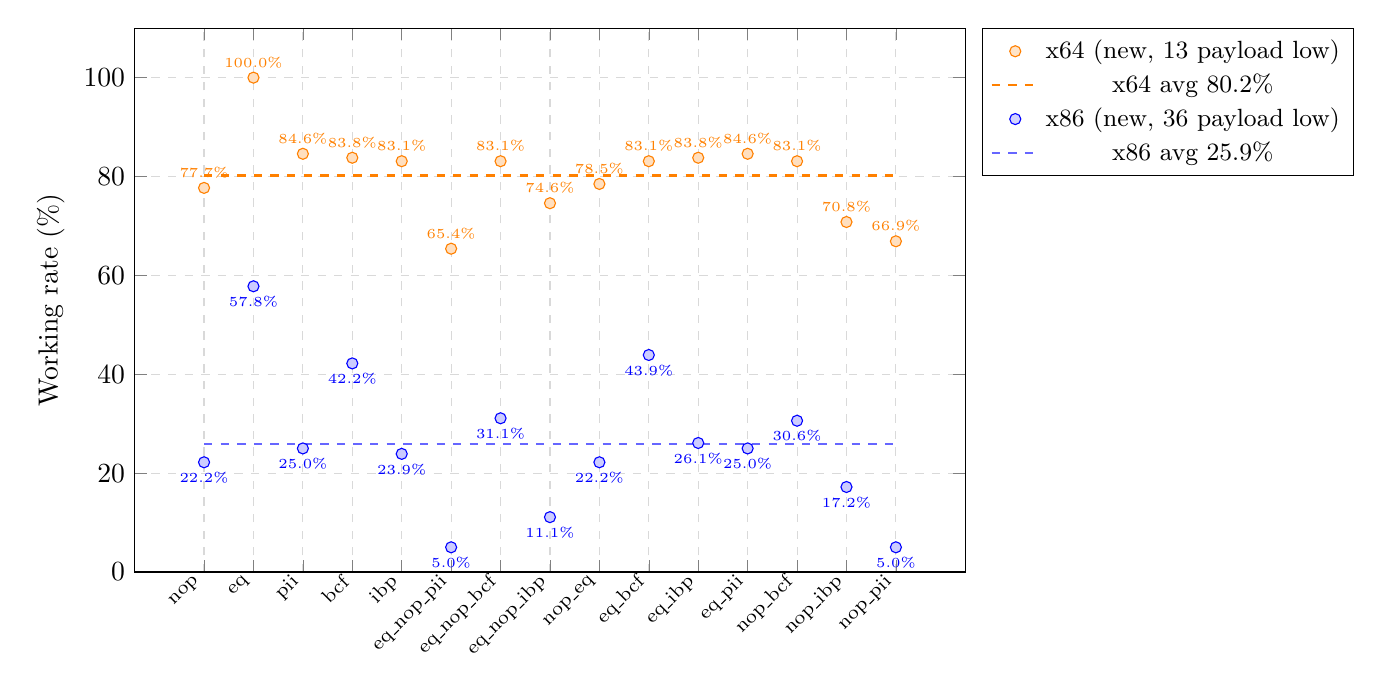
\begin{tikzpicture}
\begin{axis}[
    width=\linewidth,
    height=0.7\linewidth,
    ylabel={Working rate (\%)},
    ymin=0, ymax=110,
    ytick={0,20,40,60,80,100},
    xtick={0,...,14},
    xticklabels={nop, eq, pii, bcf, ibp, eq\_nop\_pii, eq\_nop\_bcf, eq\_nop\_ibp, nop\_eq, eq\_bcf, eq\_ibp, eq\_pii, nop\_bcf, nop\_ibp, nop\_pii},
    xticklabel style={rotate=45, anchor=east, font=\scriptsize},
    legend pos=north east,
    legend style={
        at={(1.02,1)},
        anchor=north west,
        font=\small,
        fill=white,
        fill opacity=0.85,
        draw opacity=1,
        text opacity=1
    },
    grid=major,
    grid style={dashed, gray!30},
    ymajorgrids=true,
    clip=false,
]

% Averages (unweighted mean over the 15 techniques)
\addplot[orange, dashed, thick, no marks, forget plot] coordinates {(0,80.2) (14,80.2)};
\addplot[blue!60, dashed, thick, no marks, forget plot] coordinates {(0,25.9) (14,25.9)};

% x64, new run (-xd -ebi + technique)
\addplot[only marks, mark=*, mark size=2pt, orange,
         mark options={fill=orange!25, draw=orange}]
    coordinates {(0,77.7) (1,100.0) (2,84.6) (3,83.8) (4,83.1) (5,65.4) (6,83.1) (7,74.6) (8,78.5) (9,83.1) (10,83.8) (11,84.6) (12,83.1) (13,70.8) (14,66.9)};
\addlegendentry{x64 (new, 13 payload low)}
\addlegendimage{orange, dashed, thick}
\addlegendentry{x64 avg 80.2\%}

% x86, new run
\addplot[only marks, mark=*, mark size=2pt, blue,
         mark options={fill=blue!20, draw=blue}]
    coordinates {(0,22.2) (1,57.8) (2,25.0) (3,42.2) (4,23.9) (5,5.0) (6,31.1) (7,11.1) (8,22.2) (9,43.9) (10,26.1) (11,25.0) (12,30.6) (13,17.2) (14,5.0)};
\addlegendentry{x86 (new, 36 payload low)}
\addlegendimage{blue!60, dashed, thick}
\addlegendentry{x86 avg 25.9\%}

\node at (axis cs:0,77.7) [above, orange, font=\tiny] {77.7\%};
\node at (axis cs:1,100.0) [above, orange, font=\tiny] {100.0\%};
\node at (axis cs:2,84.6) [above, orange, font=\tiny] {84.6\%};
\node at (axis cs:3,83.8) [above, orange, font=\tiny] {83.8\%};
\node at (axis cs:4,83.1) [above, orange, font=\tiny] {83.1\%};
\node at (axis cs:5,65.4) [above, orange, font=\tiny] {65.4\%};
\node at (axis cs:6,83.1) [above, orange, font=\tiny] {83.1\%};
\node at (axis cs:7,74.6) [above, orange, font=\tiny] {74.6\%};
\node at (axis cs:8,78.5) [above, orange, font=\tiny] {78.5\%};
\node at (axis cs:9,83.1) [above, orange, font=\tiny] {83.1\%};
\node at (axis cs:10,83.8) [above, orange, font=\tiny] {83.8\%};
\node at (axis cs:11,84.6) [above, orange, font=\tiny] {84.6\%};
\node at (axis cs:12,83.1) [above, orange, font=\tiny] {83.1\%};
\node at (axis cs:13,70.8) [above, orange, font=\tiny] {70.8\%};
\node at (axis cs:14,66.9) [above, orange, font=\tiny] {66.9\%};
\node at (axis cs:0,22.2) [below, blue, font=\tiny] {22.2\%};
\node at (axis cs:1,57.8) [below, blue, font=\tiny] {57.8\%};
\node at (axis cs:2,25.0) [below, blue, font=\tiny] {25.0\%};
\node at (axis cs:3,42.2) [below, blue, font=\tiny] {42.2\%};
\node at (axis cs:4,23.9) [below, blue, font=\tiny] {23.9\%};
\node at (axis cs:5,5.0) [below, blue, font=\tiny] {5.0\%};
\node at (axis cs:6,31.1) [below, blue, font=\tiny] {31.1\%};
\node at (axis cs:7,11.1) [below, blue, font=\tiny] {11.1\%};
\node at (axis cs:8,22.2) [below, blue, font=\tiny] {22.2\%};
\node at (axis cs:9,43.9) [below, blue, font=\tiny] {43.9\%};
\node at (axis cs:10,26.1) [below, blue, font=\tiny] {26.1\%};
\node at (axis cs:11,25.0) [below, blue, font=\tiny] {25.0\%};
\node at (axis cs:12,30.6) [below, blue, font=\tiny] {30.6\%};
\node at (axis cs:13,17.2) [below, blue, font=\tiny] {17.2\%};
\node at (axis cs:14,5.0) [below, blue, font=\tiny] {5.0\%};
\end{axis}
\end{tikzpicture}
\caption{Working rate by technique after regeneration with \texttt{-xd -ebi} on the
49 low-rate payloads (13 x64, 36 x86). x64: 10 runs per configuration; x86: 5 runs
per configuration. Dashed lines are the unweighted means over the 15 techniques.
Extraction only (no morphing) gives 100.0\% on x64 and 94.4\% on x86.}
\label{fig:working_rate_new}
\end{figure}

\end{document}
